\chapter{Program Development}
\label{ch:development}
\graphicspath{{image_directory/development/}}

\section{Developing Tools}

	The Python code was developed entirely in the PyCharm IDE \cite{PyCharm}, this tool allows a user to activate the GitHub version control functions and view the history log from within the editor. Python was chosen as the developing language for this tool due to its compatibility and cross platform benefits, a wide range of functionality can be achieved by importing specific modules. PyCharm allows the importing of many modules from within the editor itself. While developing it can be useful to have a terminal window and Python console at hand, both of which are integrated into PyCharm. As well as providing functional assistance the IDE provides developing tips while coding, PyCharm will suggest syntax choices for automatic fill when using special functions from modules or keywords. Keywords are easy to spot as PyCharm has a colour style (which can be change to many colour schemes) that allows numbers, function definitions, keywords and comments to be identified quickly and easily. The TFM tool developed here uses many different functions, while defining functions it is important to consider the scope of variable names used in the rest of the program, PyCharm will identify a conflicting variable name from within a function as to avoid scope error. See Figure \ref{fig:dev:pycharm} for the user interface from within the PyCharm IDE. 
	\\ \\
	All the code used to simulate traffic flow for results in Chapter \ref{ch:randd} are present on the TFM$\_$Thesis GitHub repository \cite{AndrewDixonGitHub}, available at \href{https://github.com/adj97/TFM_Thesis}{github.com/adj97/TFM$\_$Thesis}, see Figure \ref{fig:dev:github} for the homepage interface. GitHub is an opensource cloud storage system for program code of any sort. Not only are the current files stored, but a detailed history of every change to the system is noted. This is incredibly useful for adding extra features, where an entire copy of code is made and then developed on a new \emph{branch}, the new feature can then be merged back to the original copy once it has been tested, or alternatively revert back to the original. GitHub is also a useful community of developers, the Facebook of coding, if public then your repository can be viewed, reviewed, tested, cloned by any GitHub user. 

	\begin{figure}
        		\begin{minipage}{0.48\textwidth}
            		\centering
            		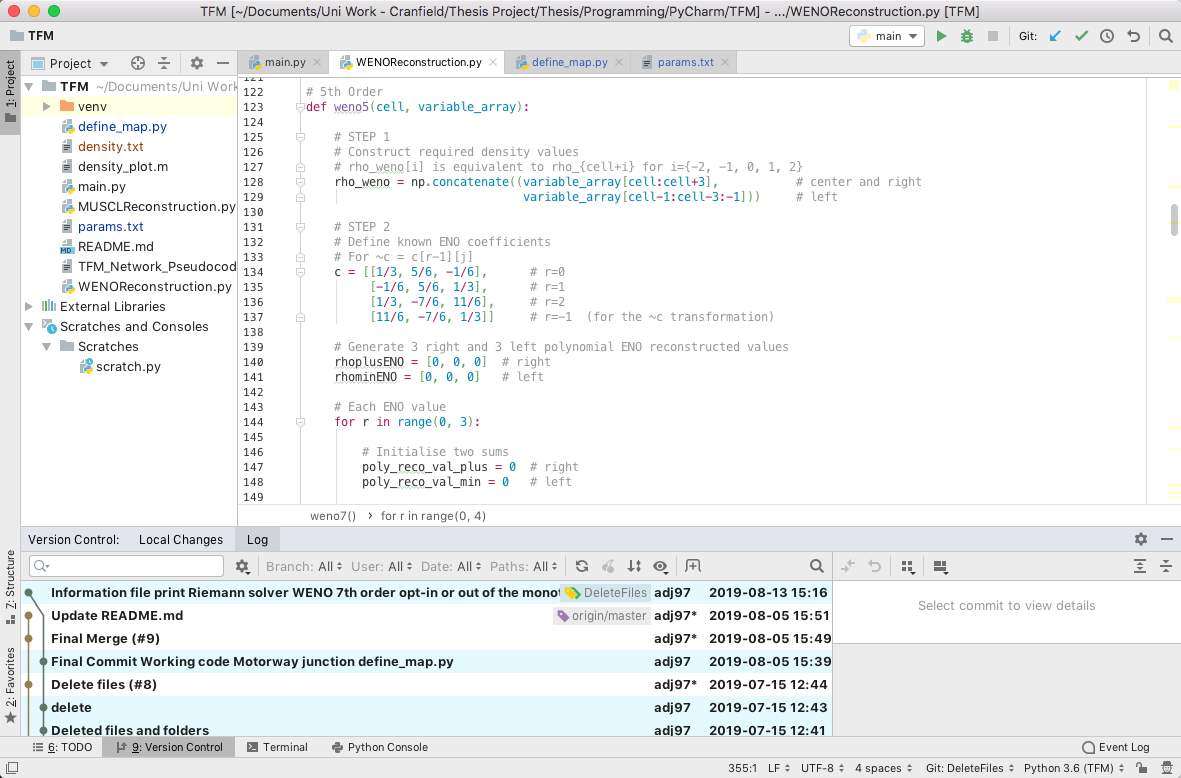
\includegraphics[trim=0 0 0 0,clip,width=\textwidth]{PyCharm.png}
            		\caption[Development : PyCharm IDE]{The multi-window GUI of the Pycharm IDE, the lower bar shows the version control log, left is the local file directory, and main window for the code editor with files open in different tabs.}
            		\label{fig:dev:pycharm}
        		\end{minipage}
        		\hfill
        		\begin{minipage}{0.48\textwidth}
            		\centering
            		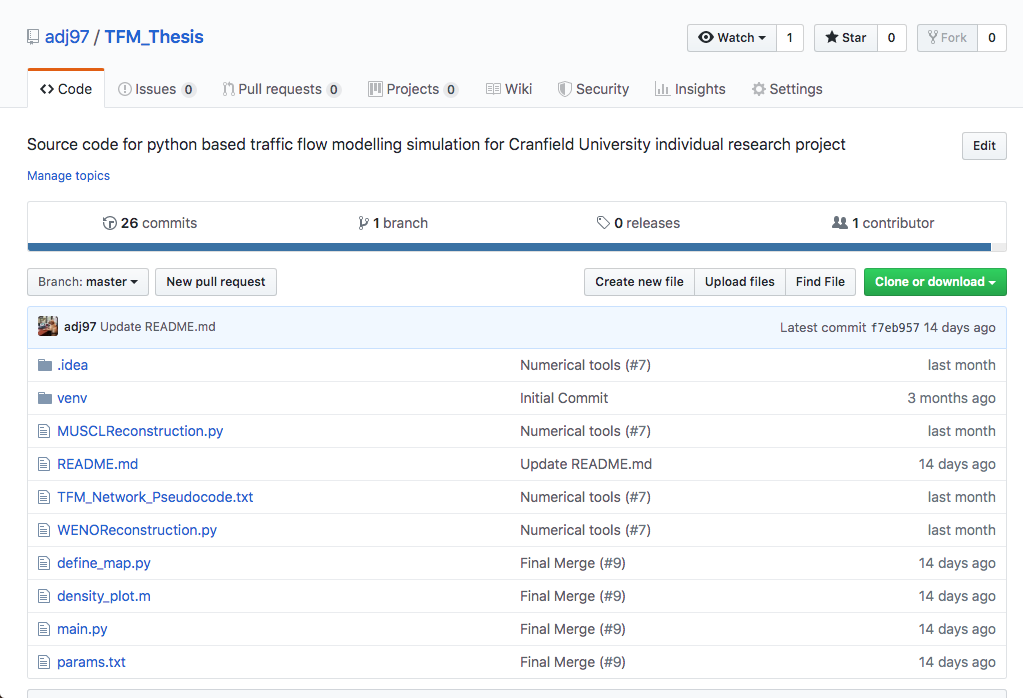
\includegraphics[trim=0 0 0 0,clip,width=0.97\textwidth]{GitHub.png}
            		\caption[Development : GitHub version control]{The TFM$\_$Thesis repository homepage, showing committed files and information on history of version control. This page links to all other features; issues, project management and all working branches.}
            		\label{fig:dev:github}
        		\end{minipage}
	\end{figure}

\section{Non-Numerical Features}

	The complex numerical procedure presented in \emph{main.py} (Appendix \ref{code:main}) is complemented by many non-numerical tools that improve ease of use, and provide extra information to the user. The following give a brief explanation to some of these features,
	\begin{itemize}
		\item Error checks and print statement - Once the program has read in the network and junction$\_$info dictionaries from \emph{define$\_$map.py}, and the parameters from \emph{params.txt}, many aspects of this input is checked for any non-compatible entries. The error types can be found in lines [55-60] of \emph{main.py} in Appendix \ref{code:main}. If any such errors are found then a breakdown of error messages and how many have occurred are printed before the program exits allowing the user to re-input information and try again. 
		\item Internal data structures - There are a wide number of arrays and data objects that have small and large features in the overall solver, listed are the main objects with a small description
		\begin{itemize}
			\item Dictionaries - Small information structures are useful to store in dictionaries as each entry will have a key tag that can be used to give meaningful names to objects.
			\item JSON file - The parameter text file is written in JavaScript Object Notation (JSON), this allows for quick and simple definition of the parameter values after being read in to the main program.
			\item Local flows - This is the output of the junction solver, which assigns each in/out road at a junction a flow value.
			\item Global flows - The local flows array feeds into this global flows array which acts every time step to define each road's supply and demand value to be used as boundary conditions in the iterated solution. 
			\item Source/Sink lists - A straight forward vector-type list of numbers defines both the road indexes of source and sink roads in two separate arrays. This is used to loop through and test if a road is a source/sink.
			\item Rho - The density solution is stored in this array, the whole network is can be stored road-by-road back to back for every cell for every road.
			\item Supply/Demand in junction solver - For the junction solver, this array provides the flow values at the end of in-roads and start of out-roads.
			\item Ghost densities - Prior to calculating the reconstructions, some high resolution schemes require values outside of the solution domain. This ghost array provides these values with symmetrical conditions at domain boundaries.
			\item Reconstructed - Looping through each cell, this array has two columns that are used to store the left and right reconstructed states for each cell.
			\item Cell fluxes - Reading from the reconstructed array (above), the chosen Riemann solver will compute from the two values of reconstruction at a cell interface. This array stores the Riemann problem approximate solution at the right hand side cell interface for each cell.
			\item Runge-Kutta arrays - Four separate lists of the density solution are stored, each represent the value after each Runge-Kutta iteration.
		\end{itemize}
		\item Function : get-start-end - This function is crucial to the data structure approach of storing the whole network solution in a single array. The function will return two indexes for the start and the end of the prescribed road of interest index.
		\item Loop progress bar - Giving the user more information on the progress of a simulation, this feature, shown in Figure \ref{fig:dev:progressbar}, is taken from \cite{TQDM} and is available at \href{https://github.com/tqdm/tqdm}{github.com/tqdm/tqdm}.
		\item Timing Segments - To provide information about the time spent in certain areas of the code, timing trackers are placed and results are printed in simulation output info (next in this list), these results are shown in Section \ref{sec:randd:timeanalysis}.
		\item Output information - Meaningful console (Appendix \ref{txt:info:console}) and information text file (Appendix \ref{txt:info:file}) print statements are provided if requested. The saved text file is placed in new created folder (named as the date and time) in the main working directory, which also includes the final density solution. This allows many simulations to be completed while not losing information on which parameters have been used to generate the solution. Included in the information file is a line count for all code contributing to the program, and a measure of the size of the final density solution output.
	\end{itemize}
	
	\begin{figure}
    		\centering
        		\fbox{
\includegraphics[trim=0 0 0 0,clip,width=0.7\textwidth]{progressbar.pdf}}
		\caption[Development : Simulation progress bar]{The information shown on the progress bar is (left to right): overall loop percentage complete, moving partial progress bar, loops completed/total number of loops, total time elapsed, estimated time remaining, loop speed in iterations per second.}
		\label{fig:dev:progressbar}
	\end{figure}
	
\section{File Structure}

	It is practical to arrange code in an organised manner, this includes splitting large code chunks into separate files and ordering each file to input or apply when necessary. The run procedure for this TFM program is to execute the \emph{main.py} code, this will call three other Python files, and read in a single parameter text file. Firstly the definition of the road network of interest is entirely contained within \emph{define$\_$map.py}, this means there is no need to alter the code in \emph{main.py} before use. The other two Python files that are used contain the MUSCL and WENO reconstruction procedures, presented as functions that take in the density array and a cell index which identifies the cell to reconstruct. These, like \emph{main.py}, need no code changes before running a simulation. Once a simulation is complete and the \emph{density.txt} output file is saved, any MATLAB postprocessing scripts can be used to analyse the results, for example splitting the array into a density profile for each road and plotting according to the road network. 
	
\section{Simulation Procedure}

\subsection{Pre-Processing}

	Prior to executing the simulation code, one needs to plan the study. The input in \emph{define$\_$map.py} requires lots of information about the roads and the junction links. It is useful to sketch a simplified diagram such as in Figure \ref{fig:networkdiagram}, which includes the direction for each road, identifies sources and sinks, and which gives indexes to each road and junction. Other information required for input are the each road length, maximum speed, and jam density. This diagram will help establish the road indexes, and allows the junctions to be identified by the road indexes of in and out roads. The only remaining aspect of network definition are each junction's individual TDM, the elements of which have constraints (See Section \ref{sec:networkmodel}) but can be estimated with rational.
	
	\begin{figure}
    		\centering
        		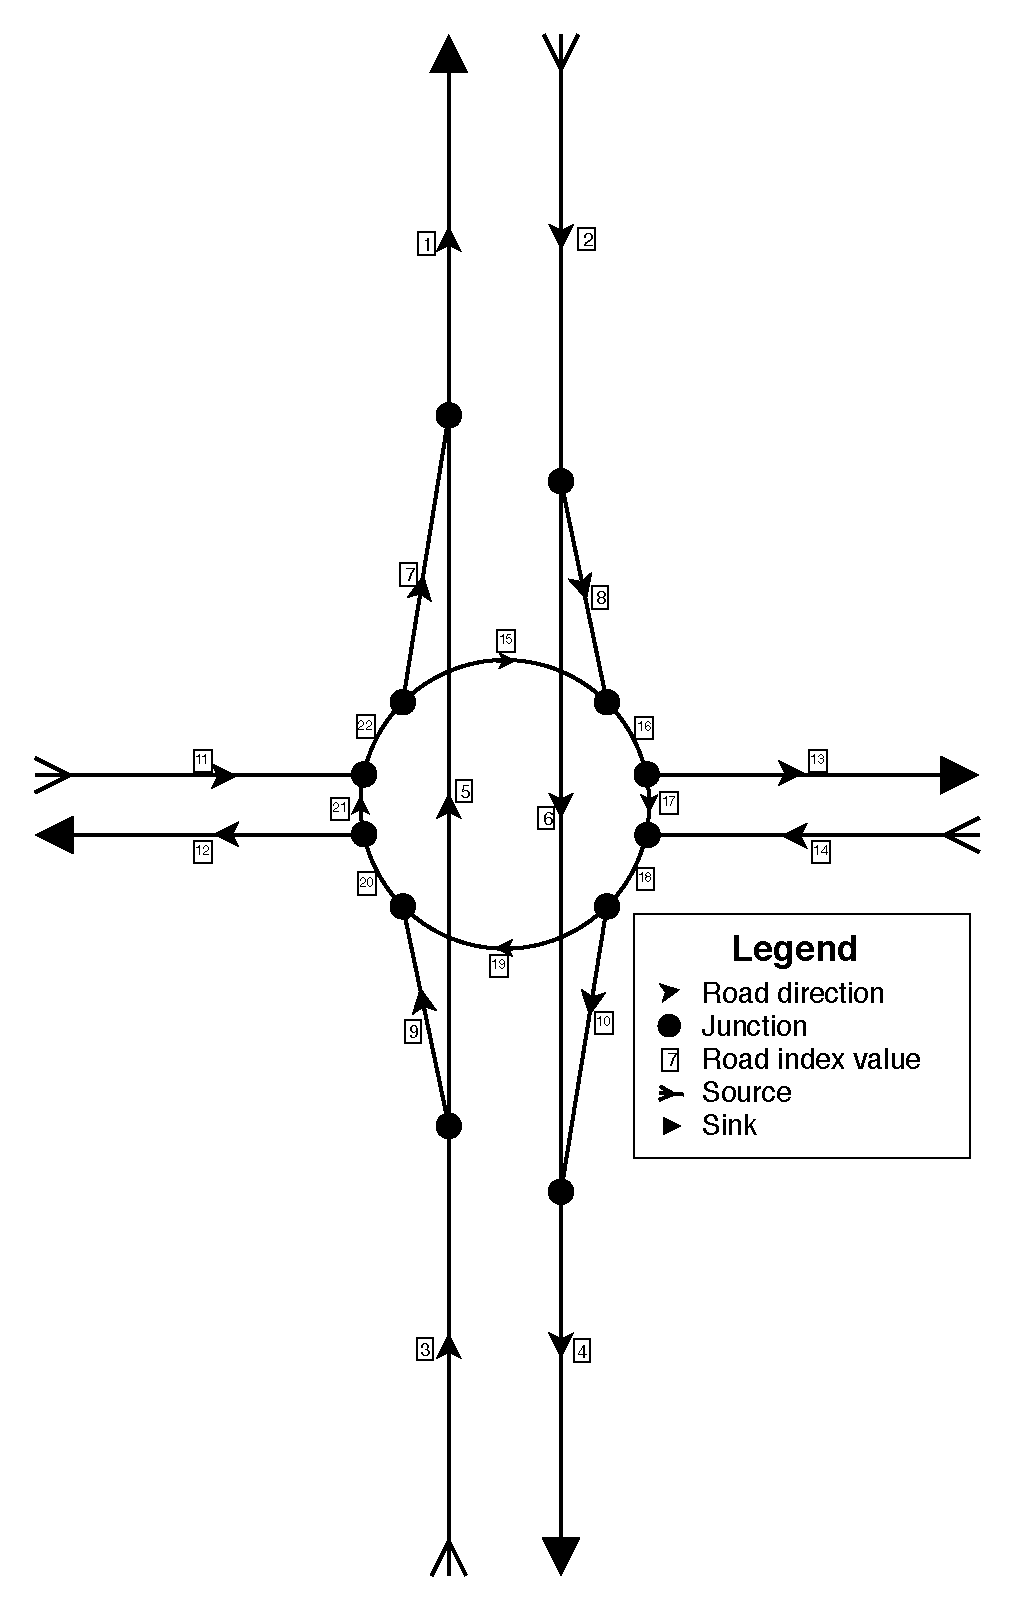
\includegraphics[trim=0 0 0 0,clip,width=0.9\textwidth]{MapDiagram.pdf}
		\caption[Development : Network map diagram]{A diagram theme for planning the definition of a road network into \emph{define$\_$map.py}, this diagram represents the Wakefield M1 junction 40 network presented in Section \ref{sec:randd:M1J40}.}
		\label{fig:networkdiagram}
	\end{figure}

\subsection{Code Algorithm}

	Once the previous steps have been carried out to define the road network of choice, the code in \emph{main.py} can be executed and the procedure outlined in Figure \ref{fig:simflowchart} will be carried out resulting in a solution profile and information file being saved to a local results folder.

	\begin{figure}
    		\centering
        		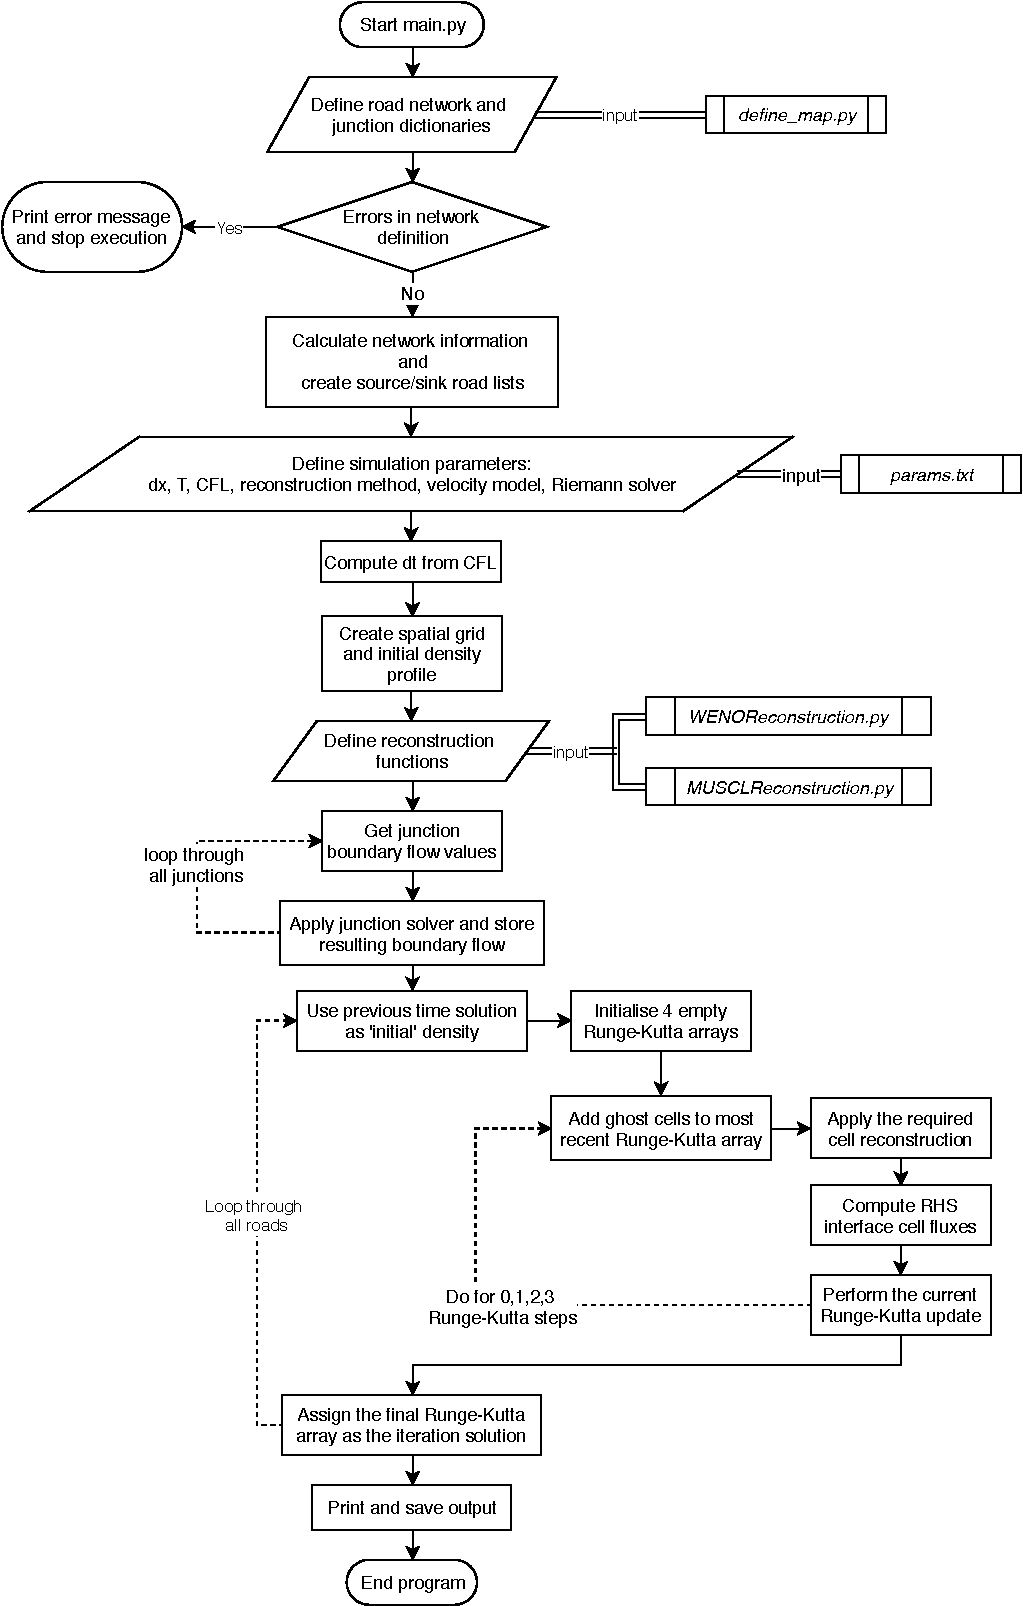
\includegraphics[trim=0 0 0 0,clip,width=\textwidth]{FlowChart.pdf}
		\caption[Development : Simulation process flowchart]{Simulation process key steps flowchart.}
		\label{fig:simflowchart}
	\end{figure}

\subsection{Postprocessing}

	The resulting \emph{density.txt} file is difficult to interpret raw; after being read in by a MATLAB script, this array can be split into many smaller objects containing the density for all time steps on a single road section each. Some example MATLAB postprocessing scripts are given in Appendix \ref{code:MATLABpostprocessing}, these can be used with no change to recreate some results of Chapter \ref{ch:randd}, or can be used as a template to develop a new script for a new road section. 